\documentclass{article}
\usepackage[utf8]{inputenc}
\usepackage{amsmath}
\usepackage{mathtools}

\usepackage{natbib}
\usepackage{graphicx}


\begin{document}

\subsection{Step One}
It is necessary to get the A-Priori distribution with an independent mean-field process. This process should be defined beforehand, to get empirical co-variance matrices and mean values. This should be done for a huge number of samples, according to the law of big numbers. The number of these samples is not the same as the number of samples for the ensemble Kalman filter. \\

\subsubsection{Euler-Approximation}

The following ODE is now chosen:
\begin{align}
    \dot{y}&=2x-4x^3, \, x\in[0,1]\\
    y(0) &= 0.
    \label{eq:DGL1}
\end{align}

The Signal $B(x)$ is now the Euler-Approximation.

\begin{align}
     \bar{X}_n^{f,(i)}&= X_{n-1}^{i}+ h\left( 2X_{n}-4X_n^3 \right) + C_n W_n^{(i)}\\
     h &= 1/50.
\end{align}

The figures \ref{fig:DGL_EF} and \ref{fig:DGL_EF2} show that the filter approaches the homogeneous solution with the starting position outlined in \ref{eq:DGL1}.

\begin{figure}[!ht]
\centering
    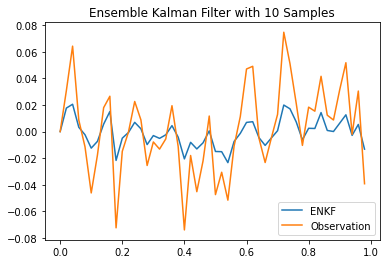
\includegraphics{M10.png}
    \caption{Linear ODE after filtering with 10 Samples and initial condition $y_0=0$, Ensemble Kalman Filter [ENKF] and noisy measurements}
    \label{fig:DGL_EF}
\end{figure}

\begin{figure}[!ht]
\centering
    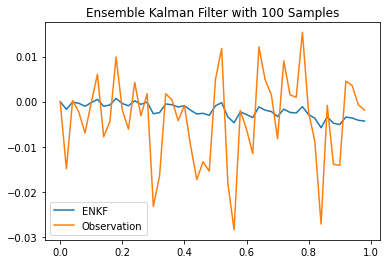
\includegraphics{M100.png}
    \caption{Linear ODE after filtering with 100 Samples and initial condition $y_0=0$, Ensemble Kalman Filter [ENKF] and noisy measurements}
    \label{fig:DGL_EF2}
\end{figure}

\begin{figure}[!ht]
\centering
    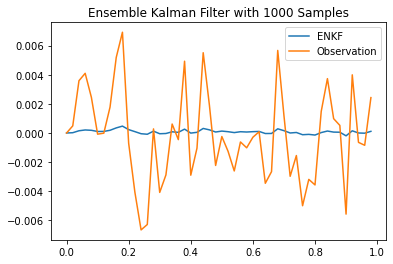
\includegraphics{M1000.png}
    \caption{Linear ODE after filtering with 1000 Samples and initial condition $y_0=0$, Ensemble Kalman Filter [ENKF] and noisy measurements}
    \label{fig:DGL_EF2}
\end{figure}


\begin{figure}[!ht]
\centering
    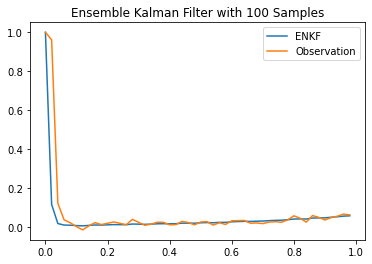
\includegraphics{M100_positive.png}
    \caption{Linear ODE after filtering with 100 Samples and initial condition $y_0=1$, Ensemble Kalman Filter [ENKF] and noisy measurements}
    \label{fig:DGL_EF3}
\end{figure}

\begin{figure}[!ht]
\centering
    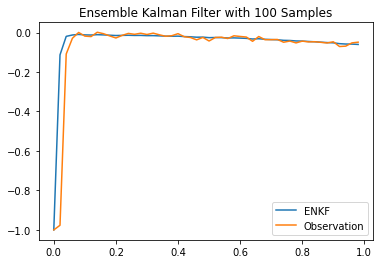
\includegraphics{M100_negative.png}
    \caption{Linear ODE after filtering with 100 Samples and initial condition $y_0=-1$, Ensemble Kalman Filter [ENKF] and noisy measurements}
    \label{fig:DGL_EF4}
\end{figure}

\subsection{Non-Linear Case}



For the non-linear case a normally distributed with mean value $0$ and standard deviation $0.6$ will be chosen as the initial state. The non-linear signal $B(x)$ will be the $cos$ function.

\begin{align}
    \bar{X}_n^{f,(i)}&= cos \left( {X}_{n-1}^{i} \right) + C_n W_n^{(i)}\\
    \bar{X}_n^{i}&= \bar{m}_n^{(i)} + T(\bar{P}_n^f) \left(\bar{X}_n^{f,(i)}-\bar{m}_n^{f} \right)
\end{align}

Samples with $M$ points were randomly chosen from the ground truth. For each number of samples, $100$ tests were performed. As seen in table \ref{tab:error}, the error is decreasing with the number of samples. 

\begin{table}[!h]
\begin{center}
\begin{tabular}{ r | c  }
  Number of Samples $M$ & Error  \\
	\hline
  10 & 0.37  \\
  100 & 0.11  \\
	1000 & 0.03
\end{tabular}
\caption{Tests for the non-linear case}
\label{tab:error}
\end{center}
\end{table}

\end{document}


